\chapter{Инструментальный пакет} \label{relWorks}

В данной главе описан инструментальный пакет, предназначенный для разработки различных решений по статическому анализу динамически формируемых выражений. Представлена архитектура разработанного инструментария, архитектура обёртки, позволяющей создавать расширения для ReSharper, предоставляющие поддержку встроенных языков. Также приведён пример конкретного расширения для ReSharper, реализованного в рамках апробации. Изложенный выше алгоритм синтаксического анализа реализован в рамках одной из компонент инструментария.

\section{Архитектура}

Практически любой язык программирования может оказаться встроенным. Даже если рассматривать только SQL, то окажется, что у него множество различных диалектов, каждый из которых имеет свои особенности. Внешним языком также может быть любой язык программирования. Трудность заключается в том, что  любое из сочетаний внешнего и встроенного языка может встретиться на практике, и задачи, которые необходимо для него решать, могут быть различными (поиск ошибок, подсчёт метрик, автоматизация трансформаций и т.д.). Реализовать универсальный инструмент, решающий все задачи для всех языков, не представляется возможным, и в связи с этим необходимо создать набор инструментов, упрощающий создание конечных решений для конкретных языков и конкретных задач. В качестве примера можно рассмотреть инструментарии для разработки компиляторов, которые включают в себя генераторы лексических, синтаксических анализаторов и набор библиотек с вспомогательными функциями, и тем самым упрощают создание конкретного компилятора для выбранного языка и целевой платформы.

Создаваемый набор инструментов должен поддерживать весь процесс обработки кода со встроенными языками, который может выглядеть так, как представлено на рисунке~\ref{fig:SeqSelProcessing}. Можно выделить следующие основные шаги.
\begin{itemize}
    \item Aнализ основного кода, который выполняется сторонним инструментом. Результат этого шага --- это дерево разбора с информацией, достаточной для выполнения дальнейших шагов.
    \item Построение аппроксимации множества возможных значений динамически формируемых выражений.
    \item Лексический анализ построенной на предыдущем шаге аппроксимации.
    \item Синтаксический анализ, результатом которого является лес разбора, пригодный для дальнейшей обработки.
    \item Обработка леса разбора, вычисление семантики.
\end{itemize}

На каждом шаге может быть получена информация, полезная для пользователя, такая как список ошибок, и её необходимо вернуть и отобразить соответствующим образом.

\begin{figure}[h!]
\begin{center}
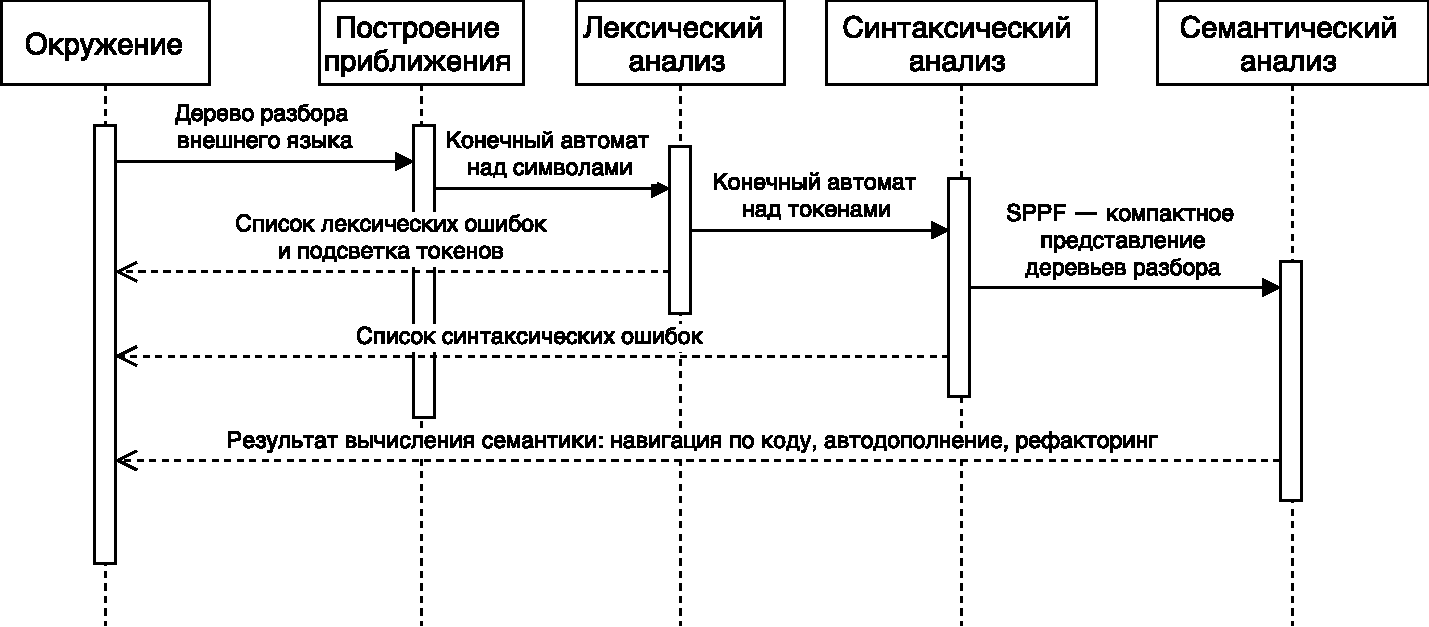
\includegraphics[width=0.9\textwidth]{pics/Seq_sel_processing_rus}
\caption{Диаграмма последовательности обработки встроенных языков}
\label{fig:SeqSelProcessing} 
\end{center}
\end{figure}

Так как анализ внешнего языка является большой самостоятельной задачей, то в рамках разработанного инструментария делается предположение, что такой анализ производится внешними инструментами. Предполагаем, что на вход можно получить дерево разбора внешнего языка с информацией, достаточной для решения поставленных в данной работе задач. Таким образом, первый шаг, выполнение которого необходимо обеспечить, --- это построение аппроксимации. В нашем случае строится регулярное приближение множества значений динамически формируемого выражения.

Для того чтобы упростить процесс создания конечных инструментов, создан пакет, одной из компонент которого является генератор синтаксических анализаторов на основе предложенного алгоритма. Также в него входит генератор лексических анализаторов, библиотека построения регулярной аппроксимации, набор вспомогательных функций.

Существующие инструменты для работы со встроенными языками реализуют поддержку какого-то одного конкретного языка, или поддержка нового языка может потребовать нетривиального ручного вмешательства. Чтобы получить поддержку встроенного языка без изменений в исходном коде инструмента, необходимо предоставить механизм для простой реализации поддержки нового языка и интеграции его в систему. Подобный механизм будет описан далее.


\subsection{Архитектура SDK}

Разработанный инструментальный пакет (SDK) включает компоненты, необходимые для реализации шагов, представленных на рисунке ~\ref{fig:SeqSelProcessing} и описанных ранее, за исключением анализа внешнего языка. Архитектура SDK изображена на рисунке~\ref{fig:SDKHLArch} и включает в себя генераторы анализаторов и различные библиотеки времени исполнения.

\begin{figure}[h!]
\begin{center}
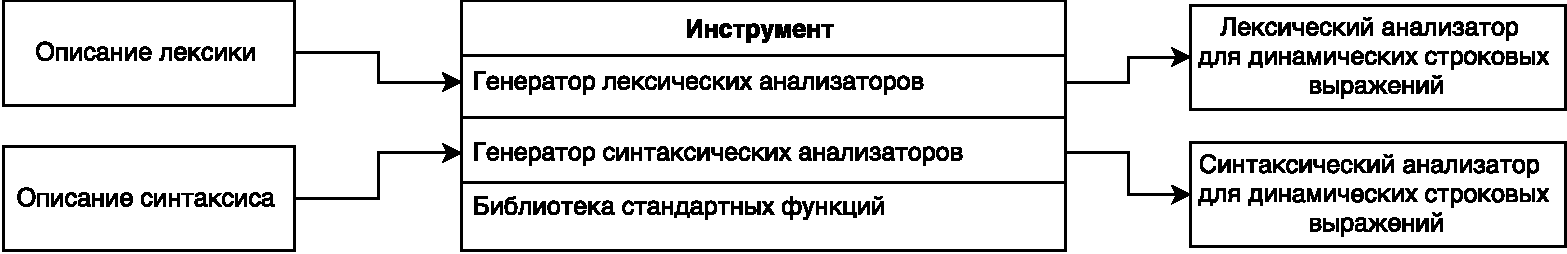
\includegraphics[width=0.9\textwidth]{pics/HighLevelArch}
\caption{Архитектура SDK целиком}
\label{fig:SDKHLArch} 
\end{center}
\end{figure}

\textbf{Построение регулярной аппроксимации} основано на алгоритме, изложенном в работе~\cite{RegOverApprox}, который позволяет строить приближение сверху для множества значений выражений. То есть $L_R$, задаваемый регулярным приближением, не меньше, чем $L_1$, задаваемый программой (выполняется включение $L_R \in L_1$). Это позволяет говорить о надёжности дальнейших анализов в том смысле, что они не теряют информации о $L_1$. Например, это важно при поиске ошибок. Если в $L_R$ не обнаружено ошибок (то есть $L_R \in L_2$, где $L_2$ --- эталонный), значит и в $L_1$ ошибок нет. При этом могут быть найдены ошибки в $L_R$, которых нет в $L_1$, то есть будут ложные срабатывания. Однако наличие ложных срабатываний лучше, чем пропущенные ошибки, и их количество может быть уменьшено путём повышения точности аппроксимации. 

Для того чтобы сделать построение приближения независимым от внешнего языка, реализовано обобщённое представление графа потока управления (Control Flow Graph, CFG)~\ref{Dragon}, которое содержит всю необходимую для дальнейшей работы информацию. Таким образом, разработчику необходимо реализовать построение обобщённого представления CFG для конкретного внешнего языка. В результате компонента строит конечный автомат, являющийся приближением множества значений динамически формируемых выражений.

Компонента, отвечающая за \textbf{лексический анализ}, состоит из двух частей: генератора лексических анализаторов, который по описанию лексики обрабатываемого языка строит соответствующий конечный преобразователь, и интерпретатора, который производит анализ входной структуры данных на основе построенного генератором преобразователя. Архитектура компоненты представлена на рисунке~\ref{fig:LexArch}. На вход принимается конечный автомат над символами, результатом работы является конечный автомат над алфавитом токенов анализируемого языка.

\begin{figure}[h!]
\begin{center}
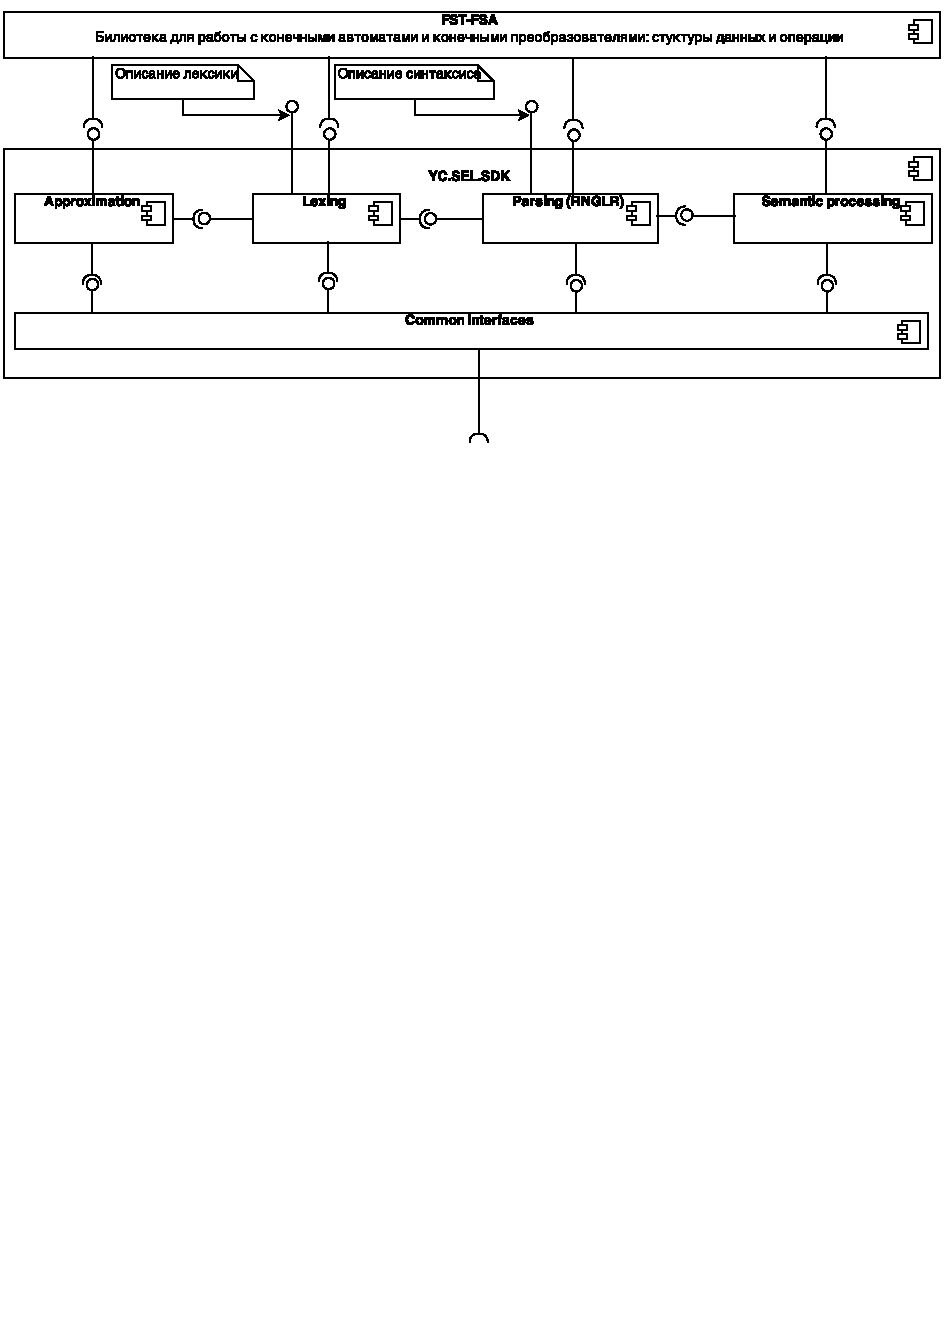
\includegraphics[width=0.9\textwidth]{pics/Components}
\caption{Архитектура лексического анализатора}
\label{fig:LexArch} 
\end{center}
\end{figure}

Лексический анализатор реализован на основе инструмента FsLex, который является стандартным генератором лексических анализаторов для языка F\#. Переиспользован язык описания лексики и некоторые структуры данных.

Реализованный генератор лексических анализаторов обладает следующими особенностями.
\begin{itemize}
    \item Поддерживаются разрывные токены, то есть ситуации, когда одна лексическая единица формируется из нескольких строковых литералов.
    \item Сохраняется привязка лексических единиц к исходному коду: сохраняется информация о строковом литерале, из которого породился токен и координаты его внутри этой строки. Так как одна лексическая единица может формироваться из нескольких строковых литералов, то привязка сохраняется отдельно для каждой части.
    \item Поддерживается обработка входных конечных автоматов, содержащих циклы.
    \item Так как значение токена может формироваться с помощью цикла и, как следствие, быть бесконечным, то каждый токен содержит конечный автомат, порождающий все возможные значения для данного токена, а не единственное значение, как это реализовано в классическом лексическом анализе.
\end{itemize}

\textbf{Генератор синтаксических анализаторов} реализован на основе алгоритма, описанного в разделе~\ref{AlgoDescr}. Его архитектура представлена на рисунке~\ref{fig:ParsArch}.  

\begin{figure}[h!]
\begin{center}
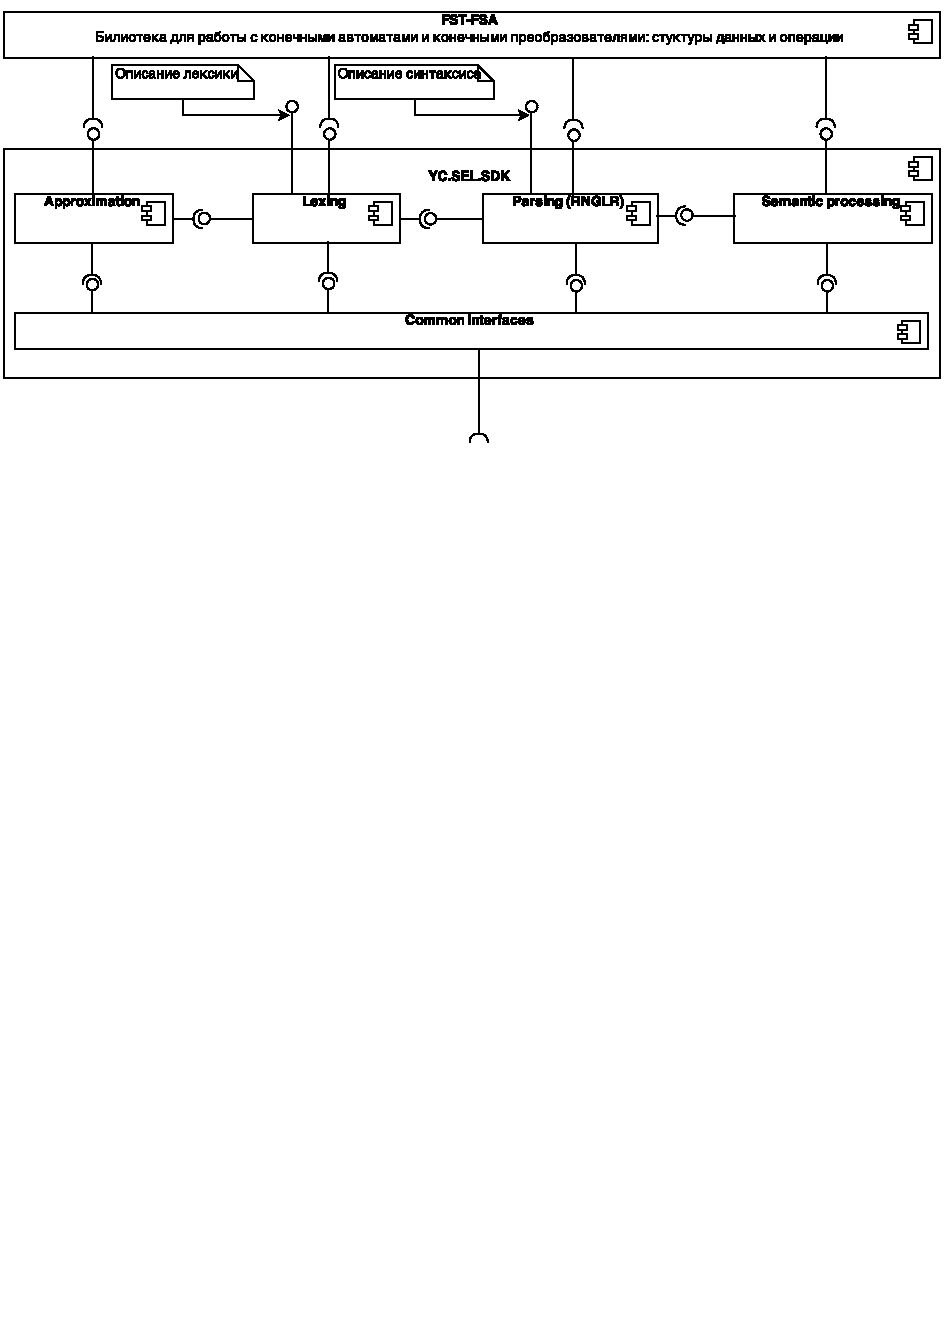
\includegraphics[width=0.9\textwidth]{pics/Components}
\caption{Архитектура синтаксического анализатора}
\label{fig:ParsArch} 
\end{center}
\end{figure}

По грамматике обрабатываемого языка строятся управляющие таблицы анализатора. Далее анализатор, реализованный в виде отдельной библиотеки, обрабатывает конечный автомат, полученный после лексического анализа. В результате будет получен SPPF, который может быть использован для дальнейшей обработки (например, подсчёта метрик). Для упрощения работы с SPPF реализован ряд вспомогательных функций.

\subsection{Архитектура расширения для ReSharper}

ReSharper --- это расширение к Microsoft Visual Studio IDE, предоставляющее широкий спектр  дополнительной функциональности по анализу и рефакторингу кода. ReSharper поддерживает несколько языков, например C\#, Visual Basic .NET, JavaScript, и этот список может быть расширен благодаря наличию свободно распространяемого ReSharper SDK, описание которого было представлено ранее в разделе~\ref{ReSharperSDKDescr}. SDK позволяет получить деревья разбора для поддерживаемых языков, предоставляет набор готовых анализов и упрощает взаимодействие с Microsoft Visual Studio IDE и её компонентами. Более того, предоставляется возможность разработки собственных расширений для ReSharper на основе SDK.

Microsoft Visual Studio является достаточно распространённой средой разработки, но не поддерживает встроенные языки, поэтому было решено разработать ряд расширений к ReSharper с использованием разработанного инструментария, которые будут устранять данный недостаток.

Стоит отметить, что не ставилось задачи поддержать все встроенные языки, так как встроенным может быть любой язык программирования. Также не было необходимости поддержать все внешние языки программирования. Необходимо на базе разработанного инструментария создать инфраструктуру, позволяющую реализовывать поддержку новых встроенных языков в Microsoft Visual   Studio через расширения к ReSharper и реализовать несколько расширений, демонстрирующих возможности созданной инфраструктуры. 

Так как необходимо поддерживать различные языки, то необходимо обеспечить расширяемость по языкам. Классический подход к решению такой задачи для интегрированных сред разработки заключается в том, что поддержка нового языка реализуется в виде независимой компоненты. Если пользователь хочет получить поддержку какого-либо языка в своей среде разработки, то он должен установить соответствующий пакет. При этом поддержка различных языков осуществляется независимо, однако часто выделяется общая функциональность, которая может быть оформлена в виде отдельного пакета.

Для предоставления описанных выше возможностей была реализована обёртка над основным SDK, упрощающая создание расширений для ReSharper. Её архитектура представлена на рисунке~\ref{fig:ReShSDKComponents}.

\begin{figure}[h!]
\begin{center}
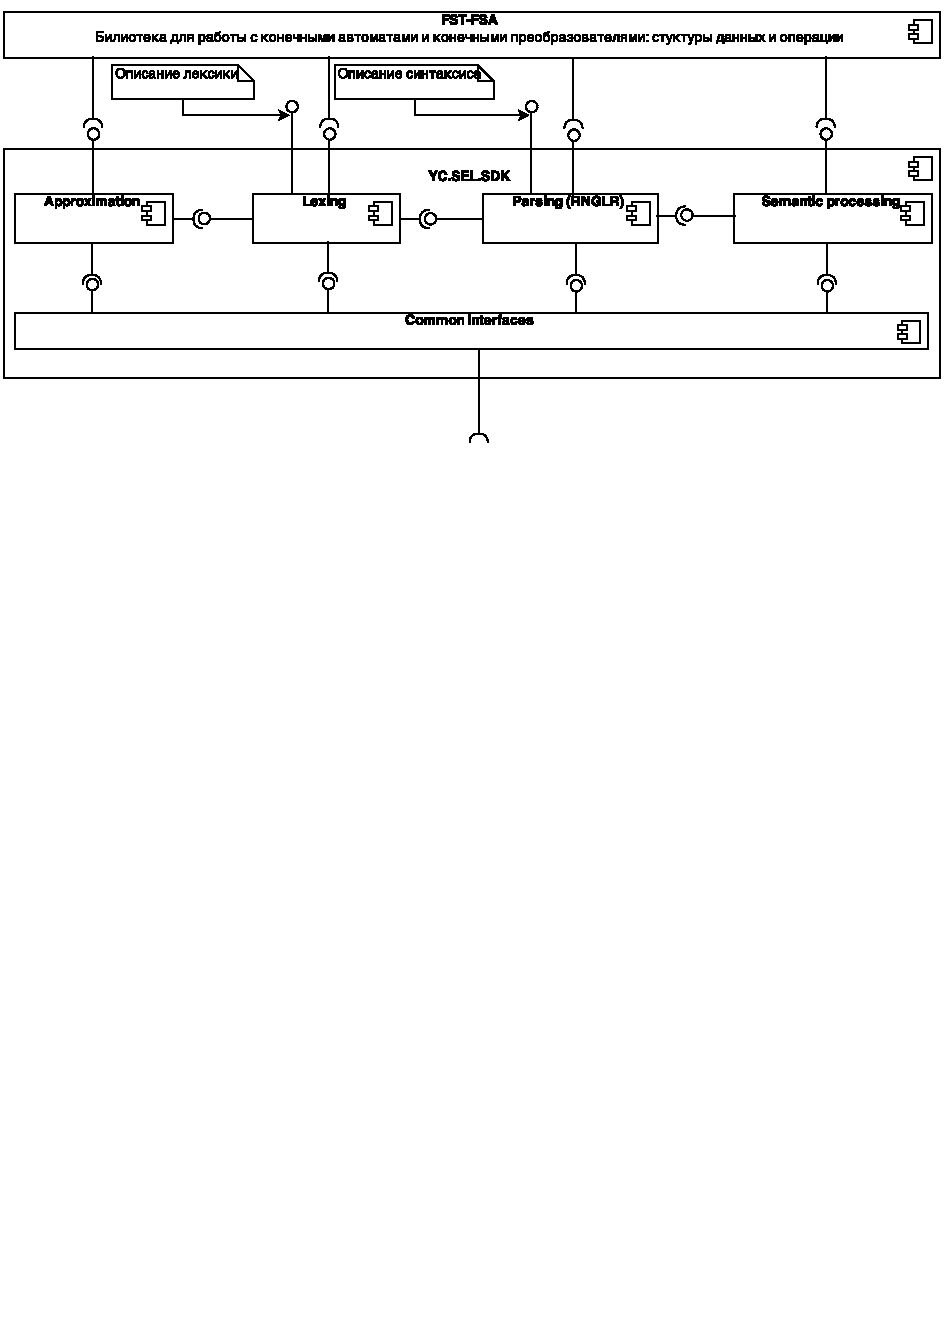
\includegraphics[width=0.9\textwidth]{pics/Components}
\caption{Архитектура инфраструктуры}
\label{fig:ReShSDKComponents} 
\end{center}
\end{figure}


\begin{figure}[h!]
\begin{center}
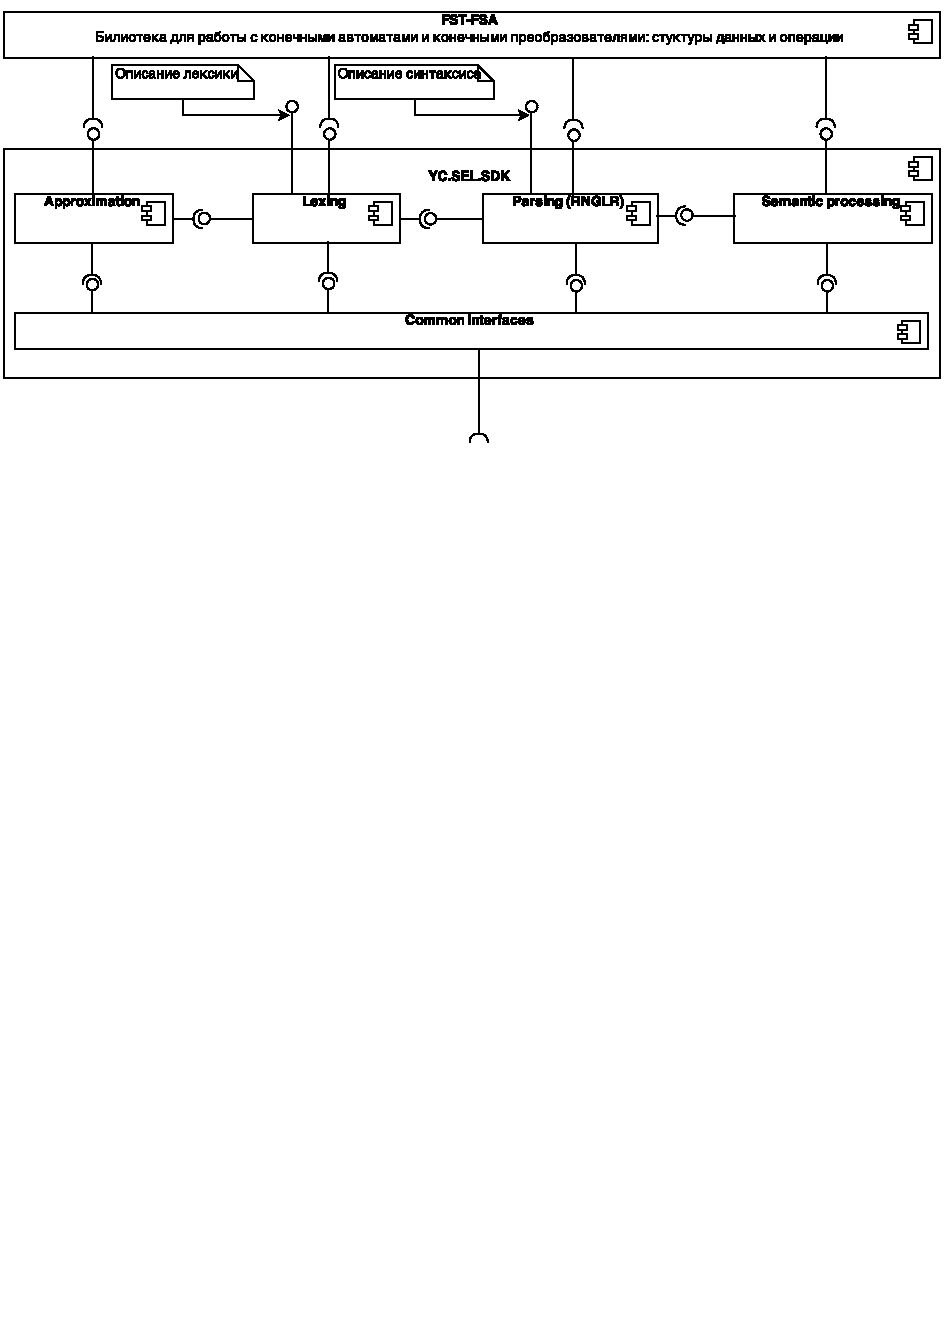
\includegraphics[width=0.9\textwidth]{pics/Components}
\caption{Архитектура конкретного плагина}
\label{fig:ReSharperPluginArch} 
\end{center}
\end{figure}

Встроенными могут быть различные языки, и учесть заранее все их особенности не представляется возможным. Кроме того, даже при использовании одного встроенного языка могут использоваться различные способы выполнения сформированного запроса. Таким образом, необходимо предоставлять возможность настройки плагинов конечным пользователем. Была реализована возможность управления следующими основными параметрами. 

\begin{itemize}
    \item Подсветка синтаксиса для каждого языка. Предоставлена возможность указать цвет для каждого типа токена.
    \item Указание парных элементов. Для каждого языка можно указать, какие лексические единицы считать парными: для каждой пары указывается ``левый'' (открывающая скобка) и ``правый'' (закрывающая скобка) элементы. При расположении курсора в тексте рядом с одним из элементов пары будут подсвечены соответсвующие элементы. Пример подсветки парных элементов приведён на рисунке~\ref{!!!!}
    \item \textbf{Точки интереса} или хотспоты (hotspot) --- это места, в которых должно быть сформировано финальное выражение. Необходимо знать, какой хотспот какому языку соответствует. При этом нужно учитывать, что одному языку может соответствовать несколько хотспотов. Например, динамически сформированный SQL-запрос в программе на языке программирования C\# может быть выполнен с помощью метода \verb|ExecuteQuery| класса \verb|DataContext|~\footnote{Документация метода \textbf{\texttt{ExecuteQuery}} (посещено 28.06.2015): \url{https://msdn.microsoft.com/en-us/library/system.data.linq.datacontext.executequery(v=vs.110).aspx}} или же текст запроса может быть передан как аргумент конструктора класса \verb|SqlCommand|~\footnote{Документация класса \textbf{\texttt{SqlCommand}} (посещено 28.06.2015): \url{https://msdn.microsoft.com/ru-ru/library/sebfsz50(v=vs.110).aspx}} с последующим выполнением с помощью метода \verb|ExecuteReader|.

\end{itemize}

Настройка указанных выше параметров хранится в соответствующих конфигурационных файлах в формате XML, которые на данный момент редактируются вручную. Настройка подсветки синтаксиса и парных элементов совмещена в одном файле и для каждого языка создаётся отдельный такой файл. Конфигурационный файл с точками интереса является общим для всех языков и, соответственно, для всех установленных расширений для поддержки встроенных языков.

В листинге~\ref{lst:codeHighlighting} приведён пример конфигурации подсветки синтаксиса и парных скобок для языка Calc. Для указания цвета используются имена, принятые в ReSharper (например \verb|"CONSTANT_IDENTIFIER_ATTRIBUTE"|), что должно сделать настройку цветов более единообразной. В xml-тэге \verb|Matched| содержится описание парных элементов. Каждая пара описывается в xml-тэге \verb|Pair| и для одного языка может быть указано более одной такой пары.

\fvset{frame=lines,framesep=5pt}
\begin{listing}[H]
    \begin{pyglist}[language=xml,numbers=left,numbersep=5pt]
<?xml version="1.0" encoding="utf-8"?>
<SyntaxDefinition name="CalcHighlighting">
    <Colors>
        <Tokens color="CONSTANT_IDENTIFIER_ATTRIBUTE">
            <Token> DIV </Token>
            <Token> LBRACE </Token>
            <Token> MINUS </Token>
            <Token> MULT </Token>
            <Token> NUMBER </Token>
            <Token> PLUS </Token>
            <Token> POW </Token>
            <Token> RBRACE </Token>
        </Tokens>
    </Colors>
<!-- Dynamic highlighting: -->
    <Matched>
        <Pair>
            <Left> LBRACE </Left>
            <Right> RBRACE </Right>
        </Pair>
<!-- You can specify more then one pair:        
        <Pair>
            <Left> LEFT_SQUARE_BRACKET </Left>
            <Right> RIGHT_SQUARE_BRACKET </Right>
        </Pair>
        <Pair>
            <Left> LEFT_FIGURE_BRACKET </Left>
            <Right> LEFT_FIGURE_BRACKET </Right>
        </Pair>
-->        
    </Matched>
</SyntaxDefinition>
    \end{pyglist}
\caption{Пример конфигурационного файла для настройки подсветки синтаксиса}
\label{lst:codeHighlighting}
\end{listing}

Листинг~\ref{lst:hotspots} содержит пример описания точек интереса. Для каждой точки интереса должна быть указана следующая информация.
\begin{itemize}
    \item Какому встроенному языку соответствует точка. Тэг \verb|Language|.
    \item Полное имя метода, являющегося точкой интереса. Тэг \verb|Method|.
    \item Порядковый номер аргумента данного метода, являющегося выражением на встроенном языке. Нумерация начинается с нуля. Тэг \verb|ArgumentPosition|. 
    \item Возвращаемый тип метода.  Тэг \verb|ReturnType|. 
\end{itemize}

\fvset{frame=lines,framesep=5pt}
\begin{listing}[H]
    \begin{pyglist}[language=xml,numbers=left,numbersep=5pt]
<?xml version="1.0" encoding="utf-8"?>
<!-- comment about body -->
<Body>
    <!-- comment about hotspot -->
  <Hotspot>
      <!-- comment about tsql -->
      <Language> TSQL </Language>
      <!-- comment about fullName -->
      <Method>Program.ExecuteImmediate</Method>
      <!-- zero-based -->
      <ArgumentPosition> 0 </ArgumentPosition>
      <!-- comment about return type -->
      <ReturnType> void </ReturnType>
  </Hotspot>
  <Hotspot>
      <Language> Calc </Language>
      <Method>Program.Eval</Method>
      <ArgumentPosition> 0 </ArgumentPosition>
      <ReturnType> int </ReturnType>
  </Hotspot>
</Body>
    \end{pyglist}
\caption{Пример конфигурационного файла для настройки точек интереса}
\label{lst:hotspots}
\end{listing}


\section{Особенности реализации}

Разработка инструментального пакета с описанной выше архитектурой и плагинов для ReSharper велась в рамках исследовательского проекта YaccConstructor (YC), описанного в разделе~\ref{YCDescr}. Разработка велась на платформе .NET и основной язык реализации --- F\#~\cite{FSharp}. Весь исходный код опубликован на GitHub: \url{https://github.com/YaccConstructor}. Большинство компонент опубликовано под ``открытой'' лицензией Apache License Version 2.0~\footnote{Одна из так называемых ``открытых'' лицензий. Сайт с текстом лицензии и сопроводительными материалами (посещено 28.06.2015): \url{http://www.apache.org/licenses/LICENSE-2.0}}. 

За основу алгоритма синтаксического анализа динамически формируемых выражений был взят реализованный в YC алгоритм синтаксического анализа RNGLR. Генератор управляющих таблиц был использован практически без модификаций, а интерпретатор был реализован отдельный. Кроме этого, общими являются некоторые структуры данных и вспомогательные функции, такие как представление леса разбора и его печать в формате DOT~\footnote{DOT --- текстовый язык описания графов. Описание языка (посещено 28.06.2015): \url{http://www.graphviz.org/doc/info/lang.html}}, представление GSS. 

Лексичекий анализ реализован на основе инструмента FsLex, который потребовал значительных доработок для того, чтобы обеспечить обработку конечного автомата, а не линейного входа. Все остальные компоненты, необходимые для статического анализа динамически формируемых выражений, такие как построение аппроксимации, вспомогательные функции для упрощения построения целевых инструментов были реализованы ``с нуля'' в рамках проекта YC.

Бинарные пакеты, содержащие основную функциональность, опубликованы в сети интернет на NuGet~\footnote{NuGet --- менеджер пакетов для платформы .NET и одноимённый ресурс для их публикации. Позволяет публиковать и устанавливать пакеты, автоматически отслеживать зависимости между ними.  Домашняя страница: \url{https://www.nuget.org/}}.
